\section{Singularidades aisladas}
\subsection{Singularidades aisladas}

Si $z_0 \in \mathbb{C}$ y $r >0$ entonces denotamos:
\[
D'(z_0, r) = \{ z \in \mathbb{C} : 0 < |z-z_0| < r\} = D(z_0, r) \setminus \{z_0\}
\]

\begin{definición}[Singularidad aislada]
    Si $f$ es una función compleja de variable compleja, diremos que $z_0 \in \mathbb{C}$ es una \textbf{singularidad aislada} de $f$ si $\exists r > 0$ tal que $f \in \mathcal{H}(D'(z_0, r))$ pero $f \notin \mathcal{H}(D(z_0, r))$.
\end{definición}

\ejemplo{
    \begin{enumerate}
        \item La función $\frac{1}{z}$ tiene una singularidad aislada en $z_0 = 0$.
        \item La función $e^{\frac{1}{z}}$ tiene una singularidad aislada en $z_0 = 0$.
        \item La función $\frac{z^2 + 1}{z(z+1)}$ tiene singularidades aisladas en $z_0 = 0$ y $z_0 = -1$.
        \item La función $\frac{1}{\sin(\frac{1}{z})}$ tiene singularidades aisladas en $z_0 = \frac{1}{n\pi}$, con $n \in \mathbb{N} \setminus \{0\}$, y en $z_0 = 0$ (no aislada).
    \end{enumerate}
}

\begin{definición}[Tipos de singularidades aisladas]
    Tenemos 3 tipos de singularidades aisladas:
    \begin{enumerate}
        \item \textbf{Singularidad evitable}: Si $\exists \lim_{z \to z_0} f(z) = L \in \mathbb{C}$, entonces se dice que $z_0$ es una singularidad evitable de $f$.
        \item \textbf{Polo}: Si $\lim_{z \to z_0} f(z) = \infty$, entonces se dice que $z_0$ es un polo de $f$.
        \item \textbf{Singularidad esencial}: Si no se cumple ninguna de las dos condiciones anteriores, es decir, si $ \nexists \lim_{z \to z_0} f(z)$, entonces se dice que $z_0$ es una singularidad esencial de $f$.
    \end{enumerate}
\end{definición}

Tenemos las siguientes propiedades:
\begin{proposición}[Caracterización de singularidades evitables]
    Sea $f \in \mathcal{H}(D'(z_0, r))$ para algún $r > 0$, entonces son equivalentes:
    \begin{enumerate}
        \item $z_0$ es una singularidad evitable de $f$.
        \item $f$ es acotada en $D'(z_0, r')$ para algún $r' \in (0, r)$.
        \item $\lim_{z \to z_0} (z-z_0)f(z) = 0$.
        \item $f$ admitte una extensión holomorfa a $D(z_0, r)$.
    \end{enumerate}
\end{proposición}

\begin{proof}
    Es evidente que $1. \implies 2. \implies 3.$.\\
    $3. \implies 4.$ por el teorema de prolongación de funciones holomorfas.\\
    $4. \implies 1.$ es evidente.
\end{proof}

\begin{proposición}[Caracterización de polos]
    Sea $f \in \mathcal{H}(D'(z_0, r))$ para algún $r > 0$, entonces son equivalentes:
    \begin{enumerate}
        \item $z_0$ es un polo de $f$.
        \item $\exists k \in \mathbb{N}$ y $\exists h \in \mathcal{H}(D(z_0, r))$ con $h(z_0) \neq 0$ tal que:
        \[
        f(z) = \frac{h(z)}{(z-z_0)^k} \quad \forall z \in D'(z_0, r)
        \]
        \item $\exists k \in \mathbb{N}$ tal que $\lim_{z \to z_0} (z-z_0)^k f(z) = L \in \mathbb{C} \setminus \{0\}$.
    \end{enumerate} \label{prop:caracterizacion_polos}
\end{proposición}

\begin{proof}
    Si $z_0$ es un polo de $f$, entonces:
    \[
    \lim_{z \to z_0} f(z) = \infty \implies 
    \exists r_1 > 0 : |f(z)| > 1 \quad \forall z \in D'(z_0, r_1) \implies
    g \equiv \frac{1}{f} \in \mathcal{H}(D'(z_0, r_1)) \text{ y } \lim_{z \to z_0} g(z) = 0
    \]
    Así, por el principio de prolongación, $g$ admite una extensión holomorfa a $D(z_0, r_1)$.\\
    Como $g(z) \neq 0 \quad \forall z \in D'(z_0, r_1)$, tenemos que $z_0$ es un cero aislado de $g$.\\
    Luego $\exists k \in \mathbb{N}$ y $\exists h_1 \in \mathcal{H}(D(z_0, r_1))$ con $h_1(z_0) \neq 0$ tal que:
    \[
    g(z) = (z-z_0)^k h_1(z) \quad \forall z \in D(z_0, r_1)
    \]
    Con lo cual:
    \[
    f(z) = 
    \frac{1}{g(z)} = 
    \frac{1}{(z-z_0)^k h_1(z)} \forall z \in D'(z_0, r_1)
    \]
    Definimos ahora:
    \[
    h(z) =
    \begin{cases}
        (z-z_0)^k f(z) & z \in D'(z_0, r_1)\\
        \frac{1}{h_1(z)} & z = z_0
    \end{cases}
    \]
    Gracias a esta definición tenemos que $h \in \mathcal{H}(D'(z_0, r_1))$ y $h$ es continua en $z_0$, luego $h \in \mathcal{H}(D(z_0, r_1))$ y $h(z_0) = \frac{1}{h_1(z_0)} \neq 0$, por lo que:
    \[
    f(z) =
    \frac{h(z)}{(z-z_0)^k} \quad \forall z \in D'(z_0, r_1)
    \]

    Tras todo esto, tenemos que $1. \implies 2.$ trivialmente, y que $2. \implies 3.$ es trivial, y finalmente $3. \implies 1.$ es evidente al ver que:
    \[
    \lim_{z \to z_0} f(z) = 
    \lim_{z \to z_0} \frac{(z-z_0)^k f(z)}{(z-z_0)^k} \underbrace{=}_{\lim_{z \to z_0} (z-z_0)^k = L \neq 0} \infty
    \]
    Usando tambien que $\lim_{z \to z_0} \frac{1}{(z-z_0)^k} = \infty$ al ser $k > 1$.
\end{proof}

\begin{definición}[Orden del polo]
    Al natural $k$ que aparece en la caracterización de los polos se le llama \textbf{orden del polo}.
\end{definición}

\subsection{Teorema de Casorati-Weierstrass y Teorema de Picard}

\begin{teorema}[Teorema de Casorati-Weierstrass]
    Sea $f \in \mathcal{H}(D'(z_0, r))$ para algún $r > 0$. Si $z_0$ es una singularidad esencial de $f$, entonces para cada $r' \in (0, r)$, la imagen $f(D'(z_0, r'))$ es densa en $\mathbb{C}$.
\end{teorema}

\begin{proof}
    Sea $r' \in (0, r)$ y supongamos que $\overline{f(D'(z_0, r'))} \neq \mathbb{C}$. Entonces:
    \[
    \exists w_0 \in \mathbb{C}, \delta > 0 : \quad \left| f(z) - w_0 \right| \geq \delta \quad \forall z \in D'(z_0, r') \implies
    \]
    \[
    g = \frac{1}{f - w_0} \in \mathcal{H}(D'(z_0, r')), \quad |g(z)| \leq \frac{1}{\delta} \quad \forall z \in D'(z_0, r') \implies
    \]
    \[
    g \text{ admite una extensión holomorfa a } D(z_0, r') \implies
    \exists \lim_{z \to z_0} g(z) = L \in \mathbb{C}
    \]
    Ahora veamos las 2 posibilidades:
    \begin{itemize}
        \item[$L \neq 0$:] 
        \[
        L =
        \lim_{z \to z_0} g(z) =
        \lim_{z \to z_0} \frac{1}{f(z) - w_0} \implies
        \lim_{z \to z_0} f(z) - w_0 = \frac{1}{L} \implies
        \exists \lim_{z \to z_0} f(z) = \frac{1}{L} + w_0 \in \mathbb{C} \implies
        \]
        \[
        z_0 \text{ es una } \textbf{singularidad evitable} \text{ de } f \text{ (contradicción).}
        \]
        \item[$L = 0$:]
        \[
        0 = \lim_{z \to z_0} g(z) =
        \lim_{z \to z_0} \frac{1}{f(z) - w_0} \implies
        \lim_{z \to z_0} f(z) - w_0 = \infty \implies
        \lim_{z \to z_0} f(z) = \infty \implies
        \]
        \[
        z_0 \text{ es un } \textbf{polo} \text{ de } f \text{ (contradicción).}
        \]
    \end{itemize}
    En cualquiera de los dos casos, $z_0$ no puede ser una singularidad esencial de $f$, lo que contradice la hipótesis.
\end{proof}

\textbf{Nota: } Existe un resultado que nos asegura aun mas.

\begin{teorema}[Teorema de Picard]
    Sea $f \in \mathcal{H}(D'(z_0, r))$, y sea $z_0$ una singularidad esencial de $f$. Entonces, $f$ toma todos los valores complejos, con a lo sumo una excepción, infinitas veces en $D'(z_0, r)$.
\end{teorema}

Usando los teoremas de Casorati-Weierstrass y otros, podemos caracterizar las aplicaciones biholomorfas de $\mathbb{C}$ en $\mathbb{C}$.

\begin{proposición}[Caracterización de las aplicaciones biholomorfas de $\mathbb{C}$ en $\mathbb{C}$]
    Si $f : \mathbb{C} \to \mathbb{C}$ es biholomorfa (holomorfa y biyectiva), entonces $f$ es un polinomio de grado 1.
\end{proposición}

\begin{proof}
    Por el teorema de la imversa, $f$ es holomorfa.
\end{proof}

\begin{definición} [Anillo]
    Sea $z_0 \in \mathbb{C}$ y $0 \leq r < R \leq \infty$. Definimos el \textbf{anillo} centrado en $z_0$ de radios $r$ y $R$ como:
    \[
        A(z_0, r, R) = \{ z \in \mathbb{C} : r < |z - z_0| < R \}
    \]
\end{definición}

Si $f$ es holomorfa en un anillo, no podemos esperar que admita representación como suma de potencias, pero veremos que admite representación como suma de serie de Laurent.

\ejemplo{
    La serie $\sum_{n=0}^{\infty} z^n$ tiene radio de convergencia 1, luego converge para $|z| < 1$, luego la serie $\sum_{n=0}^{\infty} \frac{1}{z^n}$ converge para $|z| > 1$. Si llamamos $f_1$ a su suma y $f_2$ a la suma de la serie $\sum_{n=0}^{\infty} \frac{z^n}{3^n}$, tenemos que:
    \[
        f = f_1 + f_2 \in \mathcal{H}(A(0, 1, 3))
    \]
    y 
    \[
        f(z) = f_1(z) + f_2(z) = \sum_{n=0}^{\infty} \frac{1}{z^n} + \sum_{n=0}^{\infty} \frac{z^n}{3^n} = \sum_{n=0}^{\infty} z^{-n} + \sum_{n=0}^{\infty} \frac{z^n}{3^n}
    \]
    \[
        = \sum_{n=-\infty}^{0} z^{n} + \sum_{n=0}^{\infty} \frac{z^n}{3^n} = \sum_{n=-\infty}^{\infty} c_n z^n  
    \]
    donde 
    \[
        c_n = \begin{cases}
            1 & \text{si } n \leq -1 \\
            1 + 1 = 2 & \text{si } n = 0 \\
            \frac{1}{3^n} & \text{si } n \geq 1
        \end{cases}
    \]
}

Si $(a_n)_{n \in \mathbb{N}}$ es una sucesión de números complejos, denotamos por 
\[
        \sum_{n=-\infty}^{-1} a_n = \sum_{n=1}^{\infty} a_{-n}
\]
Si $(a_n)_{n \in \mathbb{Z}}$ es una sucesión de números complejos doble, decimos que la serie $\sum_{n=-\infty}^{\infty} a_n$ converge si las series $\sum_{n=0}^{\infty} a_n$ y $\sum_{n=1}^{\infty} a_{-n}$ convergen, y en ese caso definimos la suma como:
\[
        \sum_{n=-\infty}^{\infty} a_n = \sum_{n=0}^{\infty} a_n + \sum_{n=1}^{\infty} a_{-n}
\]
Una serie de Laurent escentrada en $z_0 \in \mathbb{C}$ es una serie de la forma:
\[
        \sum_{n=-\infty}^{\infty} c_n (z - z_0)^n
\]
con $(c_n)_{n \in \mathbb{Z}}$ una sucesión doble de números complejos.

Por lo dicho anteriormente, será convergente en $\mathbb{Z}$ si las series $\sum_{n=0}^{\infty} c_n (z - z_0)^n$ y $\sum_{n=1}^{\infty} c_{-n} (z - z_0)^{-n}$ convergen.

\subsection{Serie de Laurent}

\begin{teorema} [Desarollo de la serie de Laurent]
    Sea $f \in \mathcal{H}(A(z_0, r, R))$ con $0 \leq r < R \leq \infty$. Entonces, existe una única sucesión doble $(c_n)_{n=-\infty}^{\infty} \subset \mathbb{C}$ tal que 
    \[
        f(z) = \sum_{n=-\infty}^{\infty} c_n (z - z_0)^n \quad \forall z \in A(z_0, r, R)
    \]
    donde para cada $n \in \mathbb{Z}$:
    \[
        c_n = \frac{1}{2 \pi i} \int_{C(z_0, \rho)} \frac{f(w)}{(w - z_0)^{n+1}} dw
    \]
    para cualquier $\rho$ tal que $r < \rho < R$.
\end{teorema}

\begin{proof}
    Sea $z_1 \in A(z_0, r, R)$, tomamos $r_1, R_1$ tales que $r < r_1 < |z_1 - z_0| < R_1 < R$ y consideramos las curvas $\Gamma_1$ y $\Gamma_2$ definidas como:
    \[
        \begin{matrix}
            \Gamma_1 = I \cup \gamma_1 \cup \tilde{\gamma}_1 \\
            \Gamma_2 = I^- \cup \tilde{\gamma}_2 \cup \gamma_2
        \end{matrix}
    \]
    Las curvas $\Gamma_1$ y $\Gamma_2$ son homótopas a cero en el anillo $A(z_0, r_1, R_1)$, luego por la fórmula integral de Cauchy general, tenemos
    \[
        \Ind_{\Gamma_1}(z_1) f(z_1) = \frac{1}{2 \pi i} \int_{\Gamma_1} \frac{f(w)}{w - z_1} dw
    \]
    \[
        \Ind_{\Gamma_2}(z_1) f(z_1) = \frac{1}{2 \pi i} \int_{\Gamma_2} \frac{f(w)}{w - z_1} dw
    \]
    Como $\Ind_{\Gamma_1}(z_1) = 0$ y $\Ind_{\Gamma_2}(z_1) = 1$, sumando obtenmos
    \[
        f(z_1) = \frac{1}{2 \pi i} \int_{\Gamma_1} \frac{f(w)}{w - z_1} dw + \frac{1}{2 \pi i} \int_{\Gamma_2} \frac{f(w)}{w - z_1} dw = \frac{1}{2 \pi i} \left(\int_{C(z_0, R_1)} \frac{f(w)}{w - z_1} dw - \int_{C(z_0, r_1)} \frac{f(w)}{w - z_1} dw \right)
    \] 
    Denotando $C_1 = C(z_0, R_1)$ y $C_2 = C(z_0, r_1)$, y usando 
    \[
        R_1 = |w - z_0| > |z_1 - z_0| \implies \left| \frac{z_1 - z_0}{w - z_0} \right| < 1 \implies \frac{1}{1 - \frac{z_1 - z_0}{w - z_0}} = \sum_{n=0}^{\infty} \left( \frac{z_1 - z_0}{w - z_0} \right)^n 
    \]
    Luego
    \[
        \frac{1}{w - z_1} = \frac{1}{w - z_0 + z_0 - z_1} = \frac{1}{w-z_0} \frac{1}{1 - \frac{z_1 - z_0}{w - z_0}} = \frac{1}{w - z_0} \sum_{n=0}^{\infty} \left( \frac{z_1 - z_0}{w - z_0} \right)^n
    \]
    Así tenemos que
    \[
        \frac{1}{2 \pi i} \int_{C_1} \frac{f(w)}{w - z_1} dw = \frac{1}{2 \pi i} \int_{C_1} \left(\sum_{n=0}^{\infty} \frac{f(w)}{(w - z_0)^{n+1}} (z_1 - z_0)^n \right) dw = \sum_{n=0}^{\infty} \left(\left( \frac{1}{2 \pi i} \int_{C_1} \frac{f(w)}{(w - z_0)^{n+1}} dw \right) (z_1 - z_0)^n\right) 
    \]
    \[
        = \sum_{n=0}^{\infty} c_n (z_1 - z_0)^n
    \]
    donde   
    \[
        c_n = \frac{1}{2 \pi i} \int_{C_1} \frac{f(w)}{(w - z_0)^{n+1}} dw = \frac{1}{2 \pi i} \int_{C(z_0, \rho)} \frac{f(w)}{(w - z_0)^{n+1}} dw
    \]
    aquí hemos usado el teorema de Cauchy, teniendo en cuenta que $r < \rho < R$.
    De forma análoga, podemos repetir lo mismo para $C_2$:
    \[
        r_1 = |w - z_0| < |z_1 - z_0| \implies \left| \frac{w - z_0}{z_1 - z_0} \right| < 1 \implies \frac{1}{1 - \frac{w - z_0}{z_1 - z_0}} = \sum_{n=0}^{\infty} \left( \frac{w - z_0}{z_1 - z_0} \right)^n
    \]
    Luego
    \[
        \frac{1}{w - z_1} = \frac{1}{z_1 - z_0} \frac{1}{1 - \frac{w - z_0}{z_1 - z_0}} = \frac{1}{z_1 - z_0} \sum_{n=0}^{\infty} \left( \frac{w - z_0}{z_1 - z_0} \right)^n
    \]
    Así tenemos que
    \[
        \frac{1}{2 \pi i} \int_{C_2} \frac{f(w)}{w - z_1} dw = \frac{1}{2 \pi i} \int_{C_2} \left(\sum_{n=0}^{\infty} \frac{f(w)}{(z_1 - z_0)^{n+1}} (w - z_0)^n \right) dw = \sum_{n=0}^{\infty} \left(\left( \frac{1}{2 \pi i} \int_{C_2} f(w) (w - z_0)^n dw \right) \frac{1}{(z_1 - z_0)^{n+1}}\right)
    \]
    \[
        = \sum_{n=1}^{\infty} \left(\left( \frac{1}{2 \pi i} \int_{C_2} f(w) (w - z_0)^{n-1} dw \right) (z_1 - z_0)^{-n}\right) = \sum_{n=1}^{\infty} c_{-n} (z_1 - z_0)^{-n}
    \]
    donde
    \[
        c_{-n} = \frac{1}{2 \pi i} \int_{C_2} f(w) (w - z_0)^{n-1} dw = \frac{1}{2 \pi i} \int_{C(z_0, \rho)} f(w) (w - z_0)^{n-1} dw
    \]
    Como $z_1$ era arbitrario en $A(z_0, r, R)$, y los $c_n$ no dependen de $z_1$, tenemos el resultado.\\
    Falta por probar la unicidad. Si $\exists (b_n)_{n=-\infty}^{\infty}$ tal que 
    \[
        f(z) = \sum_{n=-\infty}^{\infty} b_n (z - z_0)^n \quad \forall z \in A(z_0, r, R)
    \]
    veamos que $b_n = c_n$ para todo $n \in \mathbb{Z}$.\\
    Sea $n \in \mathbb{N}$, llamamos $C = C(z_0, \rho)$ con $r < \rho < R$. Entonces:
    \[
        2 \pi c_n = \int_{C} \frac{f(w)}{(w - z_0)^{n+1}} dw = \int_{C} \frac{1}{(w - z_0)^{n+1}} \left( \sum_{k=-\infty}^{\infty} b_k (w - z_0)^{k} \right) dw 
    \]
    \[
        = \int_{C} \left( \sum_{k=-\infty}^{\infty} \frac{b_k(w - z_0)^{k}}{(w - z_0)^{n+1}} \right) dw = \sum_{k=-\infty}^{\infty} b_k \left( \int_{C} (w - z_0)^{k - n - 1} dw \right)
    \]
    Como hay convergencia uniforme sobre $C$ se sigue
    \[
        = \sum_{k=-\infty}^{\infty} b_k (w - z_0)^{k - n - 1} dw = \sum_{k=-\infty}^{\infty} b_k \left(\int_{C} (w - z_0)^{k - n - 1} dw \right) = b_k \int_{C} 
    \]

\end{proof}

\begin{proof}
    Sea $z_1 \in A(z_0,r,R)$. Escogemos radios $r_1$ y $R_1$ tales que
    \[
        r < r_1 < |z_1 - z_0| < R_1 < R,
    \]
    y consideramos el anillo $A(z_0,r_1,R_1)$, contenido en el dominio de holomorfía de $f$.  

    En este anillo definimos dos curvas cerradas, $\Gamma_1$ y $\Gamma_2$, definidas en la siguiente figura:
    \begin{center}
        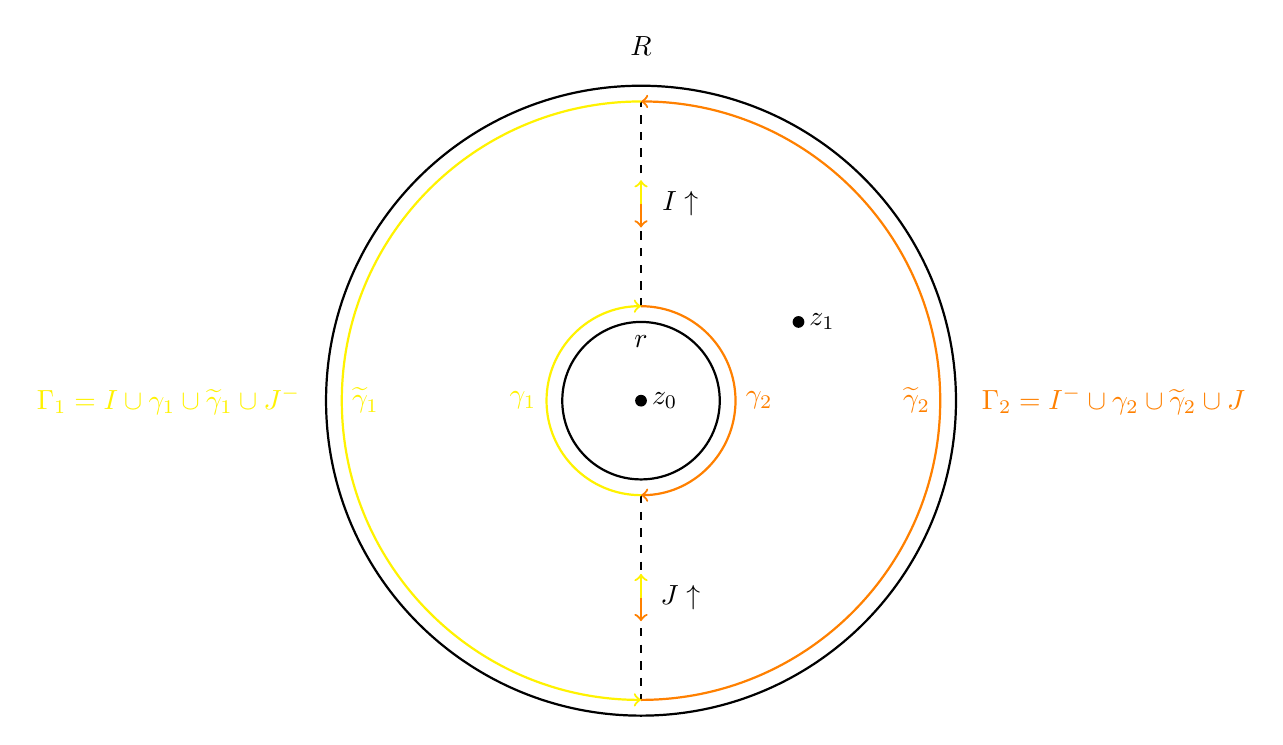
\begin{tikzpicture}
            % 4 anillos concéntricos
            \draw[thick] (0,0) circle (1cm);   % r
            %\draw[thick] (0,0) circle (1.2cm); % gamma 1,2
            %\draw[thick] (0,0) circle (3.8cm); % tilde gamma 1,2
            \draw[thick] (0,0) circle (4cm);   % R
    
            % Caminos que unen los 2 anillos intermedios por sus mitades I
            \draw[dashed] (0, 1.2) -- (0, 3.8);   % línea vertical superior
            \draw[thick, ->, yellow] (0, 2.5) -- (0, 2.8); % flecha gamma 1 - arriba
            \draw[thick, ->, orange] (0, 2.5) -- (0, 2.2); % flecha gamma 2 - abajo
            \draw[dashed] (0, -1.2) -- (0, -3.8); % línea vertical inferior
            \draw[thick, ->, orange] (0, -2.5) -- (0, -2.8); % flecha tilde gamma 2 - abajo
            \draw[thick, ->, yellow] (0, -2.5) -- (0, -2.2); % flecha tilde gamma 1 - arriba
    
            % Arco gamma 1 amarillo
            \draw[thick, ->, yellow] (0, -1.2) arc (270:90:1.2cm);
            % Arco gamma 2 naranja
            \draw[thick, ->, orange] (0, 1.2) arc (90:-90:1.2cm);
            % Arco tilde gamma 1 amarillo
            \draw[thick, ->, yellow] (0, 3.8) arc (90:270:3.8cm);
            % Arco tilde gamma 2 naranja
            \draw[thick, ->, orange] (0, -3.8) arc (270:450:3.8cm);

            % Añadimos el punto z0 en el centro
            \node at (0, 0) [circle, fill, inner sep=1.5pt] {};
            \node at (0.3, 0) {$z_0$};

            % Añadimos el punto z1 en el interior de Gamma2
            \node at (2, 1) [circle, fill, inner sep=1.5pt] {};
            \node at (2.3, 1) {$z_1$};

            
            % Nombres de las curvas con sus colores
            \node at (-1.5, 0) {\textcolor{yellow}{$\gamma_1$}};
            \node at (1.5, 0) {\textcolor{orange}{$\gamma_2$}};
            \node at (-3.5, 0) {\textcolor{yellow}{$\widetilde{\gamma}_1$}};
            \node at (3.5, 0) {\textcolor{orange}{$\widetilde{\gamma}_2$}};
    
            % Etiquetas pequeñas de los anillos
            \node at (0, 0.75) {$r$};
            \node at (0, 4.5) {$R$};
    
            % Etiquetas de las uniones entre gammas llamadas I
            \node at (0.5, 2.5) {$I \uparrow$};
            \node at (0.5, -2.5) {$J \uparrow$};
    
            % Etiquetas fuera de los anillos que indican Gamma = tilde Gamma U I U gamma U J
            \node at (-6, 0) {\textcolor{yellow}{$\Gamma_1 = I \cup \gamma_1 \cup \widetilde{\gamma}_1 \cup J^-$}};
            \node at (6, 0) {\textcolor{orange}{$\Gamma_2 = I^- \cup \gamma_2 \cup \widetilde{\gamma}_2 \cup J$}};
    
        \end{tikzpicture}
    \end{center}
    \[
        \begin{matrix}
            \Gamma_1 = I \cup \gamma_1 \cup \tilde{\gamma}_1, \\[4pt]
            \Gamma_2 = I^- \cup \tilde{\gamma}_2 \cup \gamma_2 .
        \end{matrix}
    \]
    Estas curvas son homótopas a las circunferencias $C(z_0,R_1)$ y $C(z_0,r_1)$, respectivamente, dentro del anillo $A(z_0,r_1,R_1)$.

    \medskip

    Por la fórmula integral de Cauchy generalizada obtenemos:
    \[
        \Ind_{\Gamma_1}(z_1)\, f(z_1)
        = \frac{1}{2\pi i} \int_{\Gamma_1} \frac{f(w)}{w-z_1}\, dw,
        \qquad
        \Ind_{\Gamma_2}(z_1)\, f(z_1)
        = \frac{1}{2\pi i} \int_{\Gamma_2} \frac{f(w)}{w-z_1}\, dw.
    \]
    Como $z_1$ está en el interior de $\Gamma_2$ pero en el exterior de $\Gamma_1$, se tiene:
    \[
        \Ind_{\Gamma_1}(z_1)=0, 
        \qquad
        \Ind_{\Gamma_2}(z_1)=1.
    \]
    Sumando ambas expresiones se obtiene:
    \[
        f(z_1)
        = \frac{1}{2\pi i} \left(
            \int_{\Gamma_1} \frac{f(w)}{w-z_1}\, dw
            + \int_{\Gamma_2} \frac{f(w)}{w-z_1}\, dw
            \right)
        = \frac{1}{2\pi i} \left( 
            \int_{C(z_0,R_1)} \frac{f(w)}{w-z_1}\, dw
            - \int_{C(z_0,r_1)} \frac{f(w)}{w-z_1}\, dw
        \right).
    \]
    Denotemos para simplicidad:
    \[
        C_1 = C(z_0,R_1), \qquad C_2 = C(z_0,r_1).
    \]

    %%%%%%%%%%%%%%%%%%%%%%%%
    \subsubsection*{1. Desarrollo para la parte exterior ($C_1$)}
    %%%%%%%%%%%%%%%%%%%%%%%%

    En la circunferencia exterior se cumple
    \[
        |w-z_0| = R_1 > |z_1 - z_0| \implies \left|
        \frac{z_1 - z_0}{w - z_0} \right| < 1,
    \]
    lo que permite usar la serie geométrica
    \[
        \frac{1}{1 - \frac{z_1 - z_0}{w - z_0}}
        = \sum_{n=0}^{\infty}
          \left( \frac{z_1 - z_0}{w - z_0} \right)^n.
    \]
    Por tanto:
    \[
        \frac{1}{w - z_1}
        = \frac{1}{w - z_0}
          \sum_{n=0}^{\infty}
          \left( \frac{z_1 - z_0}{w - z_0} \right)^n.
    \]

    Sustituyendo en la integral:
    \[
        \frac{1}{2\pi i} \int_{C_1} \frac{f(w)}{w - z_1}\, dw
        = \sum_{n=0}^{\infty}
          \left(
          \frac{1}{2\pi i}
          \int_{C_1} 
          \frac{f(w)}{(w - z_0)^{n+1}}\, dw
          \right)
          (z_1 - z_0)^n.
    \]
    Definimos los coeficientes
    \[
        c_n :=
        \frac{1}{2\pi i}
        \int_{C_1} \frac{f(w)}{(w - z_0)^{n+1}}\, dw
        = \frac{1}{2\pi i}
        \int_{C(z_0,\rho)} \frac{f(w)}{(w - z_0)^{n+1}}\, dw,
    \]
    donde la independencia del radio $\rho$ se obtiene por Cauchy, al estar $f$ definida en el anillo completo.

    Así, la parte exterior contribuye con
    \[
        \sum_{n=0}^{\infty} c_n (z_1 - z_0)^n.
    \]

    %%%%%%%%%%%%%%%%%%%%%%%%
    \subsubsection*{2. Desarrollo para la parte interior ($C_2$)}
    %%%%%%%%%%%%%%%%%%%%%%%%

    En la circunferencia interior se tiene
    \[
        |w - z_0| = r_1 < |z_1 - z_0|,
    \]
    lo que permite ahora expandir como
    \[
        \frac{1}{1 - \frac{w - z_0}{z_1 - z_0}}
        = \sum_{n=0}^{\infty}
          \left( \frac{w - z_0}{z_1 - z_0} \right)^n.
    \]
    De modo que
    \[
        \frac{1}{w - z_1}
        = \frac{1}{z_1 - z_0}
          \sum_{n=0}^{\infty}
          \left( \frac{w - z_0}{z_1 - z_0} \right)^n.
    \]

    Al sustituir:
    \[
        \frac{1}{2\pi i} \int_{C_2} \frac{f(w)}{w - z_1}\, dw
        = \sum_{n=0}^{\infty}
          \left(
            \frac{1}{2\pi i}
            \int_{C_2} f(w)(w - z_0)^n\, dw
          \right)
          (z_1 - z_0)^{-n-1}.
    \]
    Reindexando con $m=n+1$ obtenemos
    \[
        \sum_{m=1}^{\infty}
        \left(
        \frac{1}{2\pi i}
        \int_{C_2} f(w)(w - z_0)^{m-1}\, dw
        \right)
        (z_1 - z_0)^{-m}
        = \sum_{m=1}^{\infty} c_{-m}(z_1 - z_0)^{-m},
    \]
    donde
    \[
        c_{-m}
        = \frac{1}{2\pi i}
          \int_{C_2} f(w)(w - z_0)^{m-1}\, dw
        = \frac{1}{2\pi i}
          \int_{C(z_0,\rho)} f(w)(w - z_0)^{m-1}\, dw.
    \]

    \medskip

    %%%%%%%%%%%%%%%%%%%%%%%%
    \subsubsection*{3. Conclusión}
    %%%%%%%%%%%%%%%%%%%%%%%%

    Sumando las contribuciones interior y exterior llegamos a
    \[
        f(z_1)
        =
        \sum_{n=0}^{\infty} c_n (z_1 - z_0)^n
        +
        \sum_{n=1}^{\infty} c_{-n} (z_1 - z_0)^{-n},
    \]
    lo cual constituye exactamente el desarrollo de Laurent de $f$ en el anillo $A(z_0,r,R)$.

    La unicidad de los coeficientes $c_n$ se deduce del teorema de Cauchy y del hecho de que la representación en serie es única en un anillo conexo.

\end{proof}


\textbf{Nota:}
\begin{itemize}
    \item Falta probar la unicidad.
    \item Observamos que 
    \[
        f_1(z) := \sum_{n=0}^{\infty} c_n (z - z_0)^n \in \mathcal{H}(D(z_0, R))
    \]
    \[
        f_2(z) := \sum_{n=1}^{\infty} c_{-n} (z - z_0)^{-n} \in \mathcal{H}(\mathbb{C} \setminus \overline{D}(z_0, r))
    \]
    \item A la serie $\sum_{n=-\infty}^{-1} c_n (z - z_0)^n$ se le llama \textbf{parte principal} o \textbf{parte singular} de la serie de Laurent.
\end{itemize}

\begin{observación}
    Hemos visto en la demostración que 
    \[
        \sum_{n=0}^{\infty} (z-z_0) \in \mathcal{H}(D(z_0,R))
    \]
    y que 
    \[
        \sum_{n=1}^{\infty} c_{-n} (z - z_0)^{-n} \in \mathcal{H}(\mathbb{C} \setminus \overline{D}(z_0, r))
    \]
\end{observación}

\ejemplo{
    Halla el desarollo de Laurent de
    \[
        f(z) = \frac{1}{z(z-1)}
    \]
    en los anillos $A(0,0,1)$ y $A(0,1,\infty)$.\\
    Tenemos que
    Si $0<|z| < 1$, entonces
    \[
        \frac{1}{z} \frac{1}{z-1} = \frac{1}{z} \frac{-1}{1-z} = -\frac{1}{z} \sum_{n=0}^{\infty} z^n = -\sum_{n=0}^{\infty} z^{n-1} = -\sum_{n=-1}^{\infty} z^n
    \]
    Si $|z| > 1$, entonces $\frac{1}{|z|} < 1 \iff |\frac{1}{z}| < 1$, luego
    \[
        f(z) = \frac{1}{z} \left(\frac{1}{z-1}\right) = \frac{1}{z} \frac{1}{z} \frac{1}{1 - \frac{1}{z}} = \frac{1}{z^2} \sum_{n=0}^{\infty} \left(\frac{1}{z}\right)^n = \frac{1}{z^2} \left(1 + \frac{1}{z} + \frac{1}{z^2} + \ldots \right) = \sum_{n=-\infty}^{\infty} c_n z^n
    \]
    donde
    \[
        c_n = \begin{cases}
            0 & \text{si } n \geq -1 \\
            1 & \text{si } n \leq -2  \quad \forall z \in A(0,1,\infty)
        \end{cases}
    \]
    Otra forma de verlo es:
    \[
        f(z) = \frac{1}{z(z-1)} = -\frac{1}{z} + \frac{1}{z-1} = \frac{1}{z-1} - \frac{1}{z}
    \]  
    \[
        \begin{cases}
            g(z) = \frac{1}{z} \quad \forall z \in \mathbb{C} \setminus \{0\} \\
            h(z) = \frac{1}{z-1} = -\frac{1}{1-z} 
        \end{cases}
    \]     
}

Si $z_0$ es una singularidad aisalda de $f \in \mathcal{H}(D'(z_0, r))$, los coeficientes de la parte principal del desarrollo de Laurent de $f$ en $A(z_0, 0, r)$ nos permiten clasificar la singularidad.

\begin{proposición}
    Sea $f \in \mathcal{H}(D'(z_0, r))$ y sea $\sum_{n=-\infty}^{\infty} c_n (z - z_0)^n$ el desarrollo de Laurent de $f$ en $A(z_0, 0, r)$. Entonces:
    \begin{enumerate}
        \item $z_0$ es una singularidad evitable de $f$ si y sólo si $c_{-n} = 0$ para todo $n \in \mathbb{N}$.
        \item $z_0$ es un polo de orden $k$ de $f$ si y sólo si $c_{-k} \neq 0$ y $c_{-n} = 0$ para todo $n > k$, con $n \in \mathbb{N}$.
        \item $z_0$ es una singularidad esencial de $f$ si y sólo si $c_-n \neq 0$ para infinitos $n \in \mathbb{N}$.
    \end{enumerate}
\end{proposición}

\begin{proof}
    \leavevmode
    \begin{enumerate}
        \item $z_0$ es singularidad evitable $\iff \exists \lim_{z \to z_0} f(z) \iff f$ admite extensión holomorfa a $D(z_0, r)$.\\
        \[
            \iff f(z) = \sum_{n=0}^{\infty} c_n (z - z_0)^n \quad \forall z \in D'(z_0, r)  \iff c_{-n} = 0 \quad \forall n \in \mathbb{N}
        \]
        \item $z_0$ es polo de orden $k$ $\iff \exists h \in \mathcal{H}(D(z_0, r))$ tal que 
        \[
            f(z) = \frac{h(z)}{(z - z_0)^k} \quad \forall z \in D'(z_0, r) \quad \text{y } h(z_0) \neq 0
        \]
        luego $h(z) = (z - z_0)^k f(z)$. Como $h$ es holomorfa en $D(z_0, r)$, su desarrollo en serie de Taylor en $z_0$ es
        \[
            h(z) = \sum_{n=0}^{\infty} a_n (z - z_0)^n \quad \forall z \in D(z_0, r)
        \]
        Como $h(z_0) \neq 0 \implies a_0 \neq 0$. 
        \[
            f(z) = \frac{h(z)}{(z - z_0)^k} = \sum_{n=0}^{\infty} \frac{a_n}{(z - z_0)^{k-n}} = \sum_{n=-k}^{\infty} a_{n+k} (z - z_0)^n \quad \forall z \in D'(z_0, r)
        \]
        Definiendo $c_n = a_{n+k}$ tenemos que
        \[
            f(z) = \sum_{n=-k}^{\infty} c_n (z - z_0)^n \quad \forall z \in D'(z_0, r)
        \]
        luego por la unicidad del desarrollo de Laurent
        \[
            c_{-k} = a_0 \neq 0 \quad \text{y} \quad c_{-n} = a_{-n+k} = 0 \quad \forall n > k, n \in \mathbb{N}
        \]
        \item $z_0$ es singularidad esencial $\iff z_0$ no es una singularidad evitable ni un polo $\iff$ $c_{-k} \neq 0$ para infinitos $k \in \mathbb{N}$ (aplicando los puntos anteriores).
    \end{enumerate}
\end{proof}

\ejemplo{
    \[
        e^{\frac{1}{z}} = \sum_{n=0}^{\infty} \frac{1}{n!} \left(\frac{\frac{1}{n!}}{z^n}\right) = \sum_{n=0}^{\infty} \frac{1}{n!} z^{-n}  
    \]
    \[
        = 1 + \frac{1}{z} + \frac{1}{2! z^2} + \frac{1}{3! z^3} + \ldots
    \]
    Como $c_{-n} = \frac{1}{n!} \neq 0$ para todo $n \in \mathbb{N}$, $z=0$ es una singularidad esencial de $e^{\frac{1}{z}}$.
}

\begin{proposición}
    Si $f: \mathbb{C} \to \mathbb{C}$ es biholomorfa entonces $f$ es un polinomio de grado 1.
\end{proposición}

\begin{proof}
    Consideramos la función
    \[
        g(z) = f()
    \]
    el punto $0$ es singularidad aislada de $g$. Como $g(D(0,r))$ no es denso, no puede ser singularidad esencial. Como
    \[
        \lim_{z \to \infty} \frac{1}{g(z)} = \lim_{z \to 0} \frac{1}{f(\frac{1}{z})} = \infty
    \]
    Sea ahora:
    \[
        g(z) = f\left(\frac{1}{z}\right), \quad g: \mathbb{C} \setminus \{0\} \to \mathbb{C}
    \]
    Vimos que 0 es un polo de $g$ y que:
    \[
    \exists R > 0: \quad |g(z)| < 1 \forall z \in \mathbb{C}: |z| > R
    \]
    Así, como 0 es polo de $g$ existe un $k \in \mathbb{N}$ tal que
    \[
        h(z) = z^k g(z) \in \mathcal{H}(\mathbb{C})
    \]
    .......\\
    y además $h$ es acotada, luego:
    \[
    |h(z)| = |g(z)||z^k| < |z|^k \forall z: |z| > 1
    \]
    ......\\
    Si $z \neq 0$:
    \[
    f(z) =
    f (\frac{1}{\frac{1}{z}}) =
    g(\frac{1}{z}) =
    h(\frac{1}{z}) \frac{1}{(\frac{1}{z})^k} =
    \]
    \[
    = z^k (a_0 + a_1 \frac{1}{z} + a_2 \frac{1}{z^2} + \ldots + a_n \frac{1}{z^n}) =
    a_0 z^k + a_1 z^{k-1} + \ldots + a_n z^{k-n}
    \]
    Así $f$ es un polinomio de grado $k$. Si $k$, y como es inyectiva tenemos que $k=1$ al aplicar el teorema fundamental del algebra, luego $k=1$ y $f=a_0z$ con $a_0 \neq 0$.\\
    Si $f(0) = w_0 \neq 0$ entonces $g(z) = f(z) - w_0$ es entera y biyectiva con $g(0) = 0$, luego $g$ es un polinomio de grado 1, luego $f$ también:
    \[
    f(z) =
    g(z) + w_0 =
    a_1 z + w_0 \quad \forall z \in \mathbb{C}
    \]
\end{proof}